\documentclass[11pt]{article}
\usepackage[utf8]{inputenc}
\usepackage[T1]{fontenc}
\usepackage{amsmath}
\usepackage{amssymb}
\usepackage{graphicx}
\usepackage{geometry}
\usepackage{tikz}
\usepackage{ulem} 
\usepackage{pgfplots}
% For underline, using normalem to avoid messing with \emph
\usepackage{braket}   % For potential QM notation (optional here)

\geometry{a4paper, margin=1in}
\usetikzlibrary{positioning, arrows.meta, shapes.geometric} % For TikZ diagrams

% Custom commands (optional)
\newcommand{\avg}[1]{\overline{#1}}
\newcommand{\prob}[1]{P(#1)}
\newcommand{\ProbDens}[1]{\mathcal{P}(#1)} % Using script P for density
\newcommand{\vect}[1]{\vec{#1}}
\newcommand{\dd}[1]{\mathrm{d}#1} % Differential d
\newcommand{\pderiv}[2]{\frac{\partial #1}{\partial #2}}
\newcommand{\deriv}[2]{\frac{\mathrm{d} #1}{\mathrm{d} #2}}
\newcommand{\muState}{\mu\text{-state}} % Microstate
\newcommand{\OmegaE}{\Omega(E)}
\newcommand{\omegaE}{\omega(E)}
\newcommand{\PhiE}{\Phi(E)}
\newcommand{\deltaE}{\delta E}

\title{Physics 415 - Lecture 4}
\date{January 29, 2025}
\author{} % Author not specified

\begin{document}

\maketitle
\thispagestyle{empty}

\section*{Summary of Classical Statistical Description}

\begin{itemize}
    \item Microstate ($\mu$-state) $\leftrightarrow$ Phase space cell (size $h_0^S$).
    \item \textbf{Fundamental Postulate:} An isolated system in equilibrium is equally likely to be in any of its accessible $\mu$-states.
    \item Accessible states = $\mu$-states compatible with given constraints (e.g., energy in $(E, E+\deltaE)$).
    \item $\OmegaE$ = number of accessible states.
    \item Probability of being in a specific accessible $\mu$-state $= 1/\OmegaE$.
\end{itemize}



\section*{Quantum Mechanical (QM) Description}

In QM, the main difference from the classical approach is in the identification of $\mu$-states.
\begin{itemize}
    \item In QM, the state of a system is described by a wave function $\Psi$.
    \item Such a quantum state may be specified by a set of "quantum numbers".
\end{itemize}

\textbf{Example 1:} 1D particle in a box (Length $L$, $V=\infty$ at boundaries).
\begin{center}
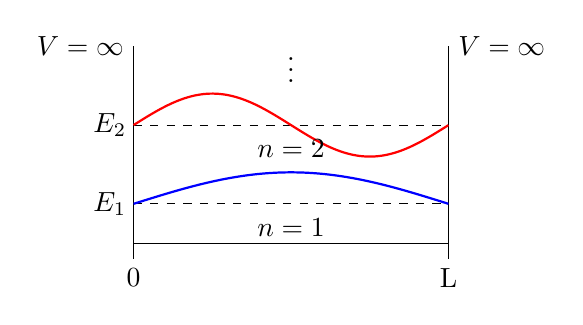
\begin{tikzpicture}
    % Box
    \draw (0,0) -- (4,0);
    \draw (0,-0.2) -- (0,2.5) node[left] {$V=\infty$};
    \draw (4,-0.2) -- (4,2.5) node[right] {$V=\infty$};
    \node at (0,-0.2) [below] {0};
    \node at (4,-0.2) [below] {L};
    % Levels
    \draw [dashed] (0,0.5) -- (4,0.5); \node at (-0.3, 0.5) {$E_1$};
    \draw [blue, thick] plot [domain=0:4, samples=100] (\x, {0.5+0.4*sin(deg(\x*pi/4))}); \node at (2, 0.2) {$n=1$};
    \draw [dashed] (0,1.5) -- (4,1.5); \node at (-0.3, 1.5) {$E_2$};
    \draw [red, thick] plot [domain=0:4, samples=100] (\x, {1.5+0.4*sin(deg(\x*2*pi/4))}); \node at (2, 1.2) {$n=2$};
    \node at (2, 2.3) {$\vdots$};
\end{tikzpicture}
\end{center}
The time-independent Schrödinger equation is:
\[ -\frac{\hbar^2}{2m} \deriv[2]{\psi}{x} = E\psi \]
with boundary conditions $\psi(x=0)=\psi(x=L)=0$.
The solutions (stationary states or $\mu$-states) are:
\begin{itemize}
    \item Wave functions: $\psi_n(x) = \sqrt{\frac{2}{L}} \sin\left(\frac{n\pi x}{L}\right)$
    \item Energies: $E_n = \frac{\hbar^2 \pi^2 n^2}{2mL^2}$
    \item Quantum number: $n=1, 2, 3, \dots$ specifies the state.
\end{itemize}

\textbf{Example 2:} 1D harmonic oscillator.
Schrödinger equation: $\left(-\frac{\hbar^2}{2m}\deriv[2]{}{x} + \frac{1}{2}kx^2\right)\psi = E\psi$.
\begin{itemize}
    \item Allowed energies: $E_n = (n + \frac{1}{2})\hbar\omega$, where $\omega = \sqrt{k/m}$.
    \item Quantum number: $n=0, 1, 2, \dots$ specifies the state.
    \item For a system of $N$ decoupled oscillators, the quantum state is specified by $N$ quantum numbers: $\{n_1, n_2, \dots, n_N\}$ with $n_i = 0, 1, 2, \dots$.
\end{itemize}

\textbf{Example 3:} Spin-1/2 particle.
Consider a spin-1/2 particle, fixed in space (no translational DOF).
\begin{itemize}
    \item The quantum state can be specified by the projection of spin along some axis (say $z$).
    \item Quantum number $m$ can take values $m = \pm 1/2$.
    \item For $N$ spin-1/2 particles fixed in space, the quantum state is specified by $N$ quantum numbers: $\{m_1, m_2, \dots, m_N\}$ with $m_i = \pm 1/2$. There are $2^N$ possible states.
\end{itemize}

\subsection*{Fundamental Postulate in QM}

In QM, the fundamental postulate is unchanged:
\begin{itemize}
    \item If $\OmegaE$ = \# of quantum states with energy in the range $(E, E+\deltaE)$ (or exactly energy $E$ if the spectrum is discrete and we consider degenerate states), then the probability that the system is in any particular accessible $\mu$-state is $1/\OmegaE$.
\end{itemize}

\textbf{Example:} Consider three spin-1/2 particles in equilibrium, in an external magnetic field $H$ (along $z$). Assume the Hamiltonian only involves the interaction with the field.
The energy of each spin depends on its $m$ value:
\[ \text{Energy} = \begin{cases} -\mu H & \text{if } m=+1/2 \\ +\mu H & \text{if } m=-1/2 \end{cases} \]
($\mu$ is the magnetic moment).
The $\mu$-states are specified by $\{m_1, m_2, m_3\}$, and there are $2^3=8$ such states in total.

Now suppose the total energy of the system is known to be exactly $E_{total} = -\mu H$.
What are the accessible states? The total energy is the sum of individual energies. We need $E_{total} = E_1 + E_2 + E_3 = -\mu H$. This requires two spins to be up ($m=+1/2$, energy $-\mu H$) and one spin to be down ($m=-1/2$, energy $+\mu H$).
The accessible states are:
\[ \{+1/2, +1/2, -1/2\}, \quad \{+1/2, -1/2, +1/2\}, \quad \{-1/2, +1/2, +1/2\} \]
There are 3 accessible states $\implies \Omega(E=-\mu H) = 3$.

\textbf{Question:} What is the probability that the first spin has $m_1 = +1/2$?
We need to count the number of accessible states where $m_1 = +1/2$. These are the first two states listed above.
$\Omega(E; m_1 = +1/2) = 2$.
The probability is $P(m_1 = +1/2) = \frac{\Omega(E; m_1 = +1/2)}{\Omega(E)} = \frac{2}{3}$.
Note also $P(m_1 = -1/2) = \frac{\Omega(E; m_1 = -1/2)}{\Omega(E)} = \frac{1}{3}$.

\textbf{Question:} What is the mean value of the magnetic moment ($\mu_z$) of the first spin?
The moment is $+\mu$ if $m_1=+1/2$ and $-\mu$ if $m_1=-1/2$.
\[ \avg{\mu_{z,1}} = P(m_1=+1/2)(+\mu) + P(m_1=-1/2)(-\mu) = \frac{2}{3}(+\mu) + \frac{1}{3}(-\mu) = \frac{1}{3}\mu \]

\section*{Density of States}

The number of accessible states $\OmegaE$ plays a central role in statistical physics. We now examine its behavior, especially when the number of DOF becomes large ($N \gg 1$).

$\OmegaE$ = \# of accessible states with energy in $(E, E+\deltaE)$.
Note that $\OmegaE$ depends on the chosen energy "width" $\deltaE$.
It is useful to write:
\[ \OmegaE = \omegaE \deltaE \]
where $\omegaE$ is the "density of states" (DOS) = \# of states per unit energy range at energy E.
$\omegaE$ is independent of $\deltaE$ (assuming $\deltaE$ is small enough that $\omegaE$ is roughly constant over the interval, but large enough to contain many states).

Another way to think about $\omegaE$:
Let $\PhiE = $ total \# of states with energy $\le E$.

\begin{center}
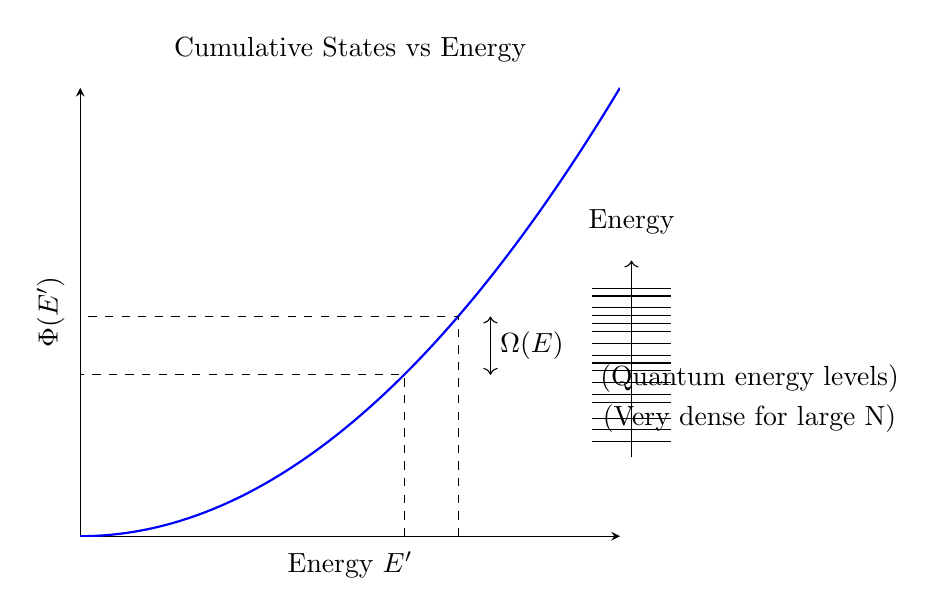
\begin{tikzpicture}
\begin{axis}[
    axis lines=left, xlabel=Energy $E'$, ylabel=$\Phi(E')$,
    xmin=0, ymin=0,
    xtick=\empty, ytick=\empty,
    title={Cumulative States vs Energy}
]
\addplot [domain=0:5, samples=100, smooth, thick, blue] {x^2}; % Example curve
\coordinate (E) at (axis cs:3, 0);
\coordinate (E_dE) at (axis cs:3.5, 0);
\coordinate (Phi_E) at (axis cs:0, 9);
\coordinate (Phi_E_dE) at (axis cs:0, 12.25);

\draw [dashed] (E) -- (E |- Phi_E) -- (Phi_E);
\draw [dashed] (E_dE) -- (E_dE |- Phi_E_dE) -- (Phi_E_dE);

\node at (E) [below] {$E$};
\node at (E_dE) [below] {$E+\deltaE$};
\node at (Phi_E) [left] {$\Phi(E)$};
\node at (Phi_E_dE) [left] {$\Phi(E+\deltaE)$};
\draw [<->] (axis cs:3.8, 9) -- (axis cs:3.8, 12.25) node [midway, right] {$\Omega(E)$};
\end{axis}
% Quantum levels illustration
\begin{scope}[xshift=7cm, yshift=1cm]
    \node at (0, 3) {Energy};
    \draw [->] (0,0) -- (0, 2.5);
    \foreach \y in {0.2, 0.35, 0.5, 0.7, 0.8, 0.95, 1.1, 1.2, 1.3, 1.45, 1.6, 1.7, 1.8, 1.9, 2.05, 2.15} {
        \draw (-0.5, \y) -- (0.5, \y);
    }
    \node at (1.5, 1) {(Quantum energy levels)};
    \node at (1.5, 0.5) {(Very dense for large N)};
\end{scope}
\end{tikzpicture}
\end{center}

When the number of particles is large, energy levels are very dense, and we can treat $\PhiE$ as a smooth function of $E$.
Then $\Omega(E) = \Phi(E+\deltaE) - \Phi(E)$.
For small $\deltaE$:
\[ \Omega(E) \approx \deriv{\PhiE}{E} \deltaE \]
Comparing with $\OmegaE = \omegaE \deltaE$, we have:
\[ \omegaE = \deriv{\PhiE}{E} \]

\subsection*{Dependence of $\OmegaE$ (or $\omegaE$) on $E$ and $N$}

How does $\OmegaE$ depend on energy $E$ and number of particles $N$ in a macroscopic system?

\textbf{Example:} Classical monatomic ideal gas.
\begin{itemize}
    \item "Monatomic": particles have no internal DOF (like rotation or vibration).
    \item "Ideal gas": neglect interactions between atoms.
\end{itemize}
Consider $N$ monatomic particles enclosed in volume $V$. The Hamiltonian is purely kinetic:
\[ H(\vec{x}_1, \dots, \vec{x}_N, \vec{p}_1, \dots, \vec{p}_N) = \sum_{i=1}^N \frac{|\vec{p}_i|^2}{2m} \]
We want the number of states $\OmegaE$ with energy in $(E, E+\deltaE)$. This corresponds to the volume of phase space satisfying:
\[ E \le \sum_{i=1}^N \frac{|\vec{p}_i|^2}{2m} \le E+\deltaE \]
The phase space volume element is $\dd{^3\vec{x}_1} \dots \dd{^3\vec{x}_N} \dd{^3\vec{p}_1} \dots \dd{^3\vec{p}_N}$.
The volume is:
\[ \text{Vol}(E, \deltaE) = \int_{E \le H \le E+\deltaE} \dd{^{3N}\vec{x}} \dd{^{3N}\vec{p}} \]
The inequality defining the integration region only depends on momenta $\vec{p}_i$, not coordinates $\vec{x}_i$. The integral over coordinates gives:
\[ \int \dd{^3\vec{x}_1} \dots \dd{^3\vec{x}_N} = \left( \int \dd{^3\vec{x}} \right)^N = V^N \]
So, the phase space volume is:
\[ \text{Vol}(E, \deltaE) = V^N \int_{E \le \sum \frac{p_i^2}{2m} \le E+\deltaE} \dd{^{3N}\vec{p}} \]
The integral is over the volume of a shell in $3N$-dimensional momentum space. The condition $\sum_i \frac{|\vec{p}_i|^2}{2m} = \mathcal{E}$ defines a hypersphere. Let $P_i = \sqrt{2m\mathcal{E}_i}$ be related momenta, then $\sum P_i^2 = 2m\mathcal{E}$. The surface $\sum_{j=1}^{3N} p_j^2 = 2m\mathcal{E}$ corresponds to a sphere of radius $R = \sqrt{2m\mathcal{E}}$ in $3N$-dimensional momentum space.

The volume of a $D$-dimensional sphere of radius $R$ is $V_D(R) = C_D R^D$ for some constant $C_D$.
Here $D=3N$. The volume in momentum space with total energy $\le \mathcal{E}$ is proportional to $(\sqrt{2m\mathcal{E}})^{3N} \propto \mathcal{E}^{3N/2}$.
Let $\text{Vol}_p(\mathcal{E})$ be the volume of momentum space with energy $\le \mathcal{E}$.
$\text{Vol}_p(\mathcal{E}) = K \mathcal{E}^{3N/2}$ for some constant $K$.
The volume of the shell between $E$ and $E+\deltaE$ is:
\[ \text{Vol}_p(E+\deltaE) - \text{Vol}_p(E) \approx \deriv{(\text{Vol}_p)}{E} \deltaE = K \left(\frac{3N}{2}\right) E^{3N/2 - 1} \deltaE \]
So the phase space volume is $\text{Vol}(E, \deltaE) \propto V^N E^{3N/2 - 1} \deltaE$.

The number of states is this volume divided by the volume of a single cell ($h_0^{3N}$ or simply $h^{3N}$ if $h_0=h$):
\[ \OmegaE \propto V^N E^{3N/2 - 1} \deltaE \]
The density of states is:
\[ \omegaE = \frac{\OmegaE}{\deltaE} \propto V^N E^{3N/2 - 1} \]
For macroscopic systems, $N \sim 10^{23}$ is very large. In this limit $3N/2 - 1 \approx 3N/2$. The notes simplify this to:
\[ \OmegaE \propto V^N E^{3N/2} \deltaE \quad (N \gg 1) \]
\[ \omegaE \propto V^N E^{3N/2} \quad (N \gg 1) \]
(Note: This captures the dominant dependence but ignores the -1 in the exponent derived above).

Key takeaway: $\OmegaE$ (and $\omegaE$) are extremely rapidly increasing functions of energy $E$. They also increase exponentially with the number of particles $N$.
This is representative of the general situation for macroscopic systems. In general:
\[ \omegaE \sim E^{Na} \]
where $a$ is a number of order 1 (e.g., $a=3/2$ for the ideal gas).

\end{document}